%% 
%% Copyright 2007-2025 Elsevier Ltd
%% 
%% This file is part of the 'Elsarticle Bundle'.
%% ---------------------------------------------
%% 
%% It may be distributed under the conditions of the LaTeX Project Public
%% License, either version 1.3 of this license or (at your option) any
%% later version.  The latest version of this license is in
%%    http://www.latex-project.org/lppl.txt
%% and version 1.3 or later is part of all distributions of LaTeX
%% version 1999/12/01 or later.
%% 
%% The list of all files belonging to the 'Elsarticle Bundle' is
%% given in the file `manifest.txt'.
%% 
%% Template article for Elsevier's document class `elsarticle'
%% with numbered style bibliographic references
%% SP 2008/03/01
%% $Id: elsarticle-template-num.tex 272 2025-01-09 17:36:26Z rishi $
%%
\documentclass[preprint,12pt]{elsarticle}

%% Use the option review to obtain double line spacing
%% \documentclass[authoryear,preprint,review,12pt]{elsarticle}

%% Use the options 1p,twocolumn; 3p; 3p,twocolumn; 5p; or 5p,twocolumn
%% for a journal layout:
%% \documentclass[final,1p,times]{elsarticle}
%% \documentclass[final,1p,times,twocolumn]{elsarticle}
%% \documentclass[final,3p,times]{elsarticle}
%% \documentclass[final,3p,times,twocolumn]{elsarticle}
%% \documentclass[final,5p,times]{elsarticle}
%% \documentclass[final,5p,times,twocolumn]{elsarticle}

%% For including figures, graphicx.sty has been loaded in
%% elsarticle.cls. If you prefer to use the old commands
%% please give \usepackage{epsfig}

%% The amssymb package provides various useful mathematical symbols
\usepackage{amssymb}
%% The amsmath package provides various useful equation environments.
\usepackage{amsmath}
%% The amsthm package provides extended theorem environments
%% \usepackage{amsthm}
\usepackage{array}
\usepackage{tabularx}
\usepackage{booktabs}
\usepackage{algorithm}
\usepackage{algorithmic}
%% The lineno packages adds line numbers. Start line numbering with
%% \begin{linenumbers}, end it with \end{linenumbers}. Or switch it on
%% for the whole article with \linenumbers.
%% \usepackage{lineno}

\journal{Journal of Theoretical Biology}

\begin{document}

\begin{frontmatter}

%% Title, authors and addresses

%% use the tnoteref command within \title for footnotes;
%% use the tnotetext command for theassociated footnote;
%% use the fnref command within \author or \affiliation for footnotes;
%% use the fntext command for theassociated footnote;
%% use the corref command within \author for corresponding author footnotes;
%% use the cortext command for theassociated footnote;
%% use the ead command for the email address,
%% and the form \ead[url] for the home page:
%% \title{Title\tnoteref{label1}}
%% \tnotetext[label1]{}
%% \author{Name\corref{cor1}\fnref{label2}}
%% \ead{email address}
%% \ead[url]{home page}
%% \fntext[label2]{}
%% \cortext[cor1]{}
%% \affiliation{organization={},
%%             addressline={},
%%             city={},
%%             postcode={},
%%             state={},
%%             country={}}
%% \fntext[label3]{}

\title{Stability-Driven Stochastic Assembly}

%% use optional labels to link authors explicitly to addresses:
%% \author[label1,label2]{}
%% \affiliation[label1]{organization={},
%%             addressline={},
%%             city={},
%%             postcode={},
%%             state={},
%%             country={}}
%%
%% \affiliation[label2]{organization={},
%%             addressline={},
%%             city={},
%%             postcode={},
%%             state={},
%%             country={}}

\author{Dan Adler} %% Author name

%% Author affiliation
\affiliation{email={dan@danadler.com}}

%% Abstract
\begin{abstract}
%% Text of abstract
The emergence of complexity and information is a fundamental question spanning disciplines from physics to biology and computation. Although traditional approaches often describe information as an emergent property, they leave unresolved how it dynamically arises from purely abiotic processes. This paper introduces Stability-Driven Stochastic Assembly (SDSA) systems, an abstract framework that models the evolution of patterns through probabilistic interactions and stability-driven selection. By abstracting away specific physical laws, SDSA systems offer a universal mechanism for generating order and information. Extending the principles of Assembly Theory (AT), SDSA systems emphasize forward dynamics, where selection pressures favor stable configurations that persist and interact more frequently. These dynamics provide a basis for understanding processes that could underlie the transition from abiotic to biotic evolution. Furthermore, the framework highlights the interplay between top-down and bottom-up causation, demonstrating how emergent patterns recursively influence their formation while being shaped by local interactions. This study offers a computationally realizable model for exploring the evolution of information, bridging the gap between randomness and complexity, while inviting further investigation into its applicability to natural and engineered systems.
\end{abstract}

%%Graphical abstract
\begin{graphicalabstract}
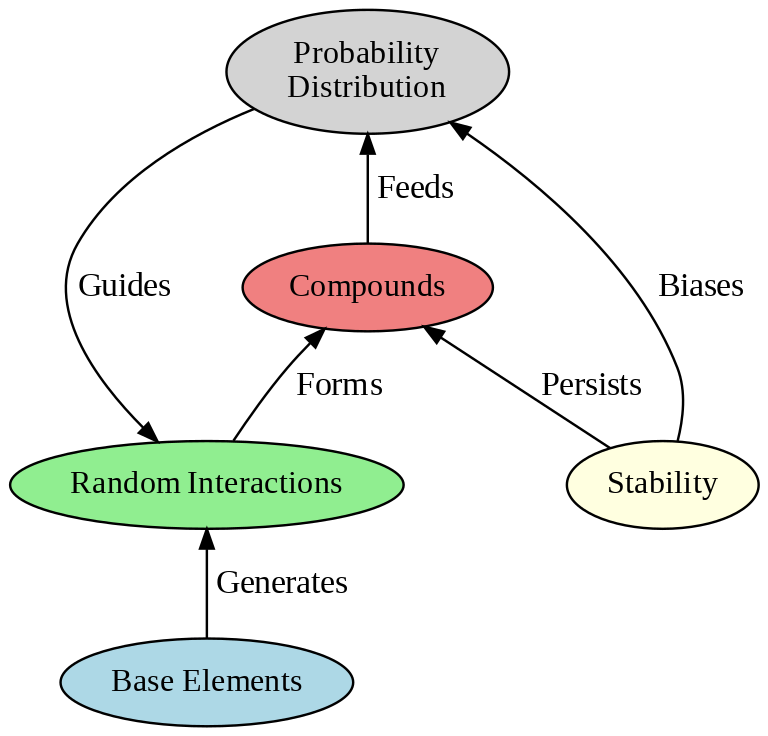
\includegraphics[width=1\textwidth]{figure_10}
\end{graphicalabstract}

%%Research highlights
\begin{highlights}
\item Develops Stability-Driven Stochastic Assembly (SDSA) as a rigorous mathematical framework for stability-based selection.
\item Formalizes how differential pattern persistence drives system evolution without requiring replication.
\item Demonstrates through precise simulations how complexity emerges from stability-driven pattern selection.
\item Quantifies the causal relationship between pattern stability and evolutionary outcomes in mixed populations.
\item Provides testable predictions for pattern formation in prebiotic and chemical evolution.
\end{highlights}

%% Keywords
\begin{keyword}
Assembly Theory; Abiotic evolution; Emergent complexity; Information Evolution; Entropy reduction; Prebiotic systems
 %% keywords here, in the form: keyword \sep keyword

%% PACS codes here, in the form: \PACS code \sep code

%% MSC codes here, in the form: \MSC code \sep code
%% or \MSC[2008] code \sep code (2000 is the default)

\end{keyword}

\end{frontmatter}

% The order of the section titles is different for some journals. Please refer to the "Instructions for Authors” on the journal homepage.

\section{Introduction}

"\textit{Selection for longevity becomes inseparable from selection for propagation. What persists has, by definition, a greater opportunity to propagate its structure.}" This observation by Stuart Kauffman \cite{kauffman1995home} identifies a fundamental principle that may bridge the gap between inanimate physical processes and biological evolution. The transition from non-living to living systems represents one of science's most profound questions, yet while the mechanisms of biological evolution through natural selection are well established, the emergence of selection itself—prior to true replication—remains enigmatic.

In inanimate physical systems, patterns persist according to their stability under prevailing conditions. A carbon lattice in diamond form persists longer than graphite under high pressure; certain molecular configurations outlast others in various chemical environments. This differential persistence creates an implicit selection mechanism—stable configurations naturally become more prevalent over time simply by outlasting less stable alternatives. This fundamental principle of stability-driven selection may have preceded and enabled the emergence of biological selection.

The study of such selection mechanisms spans multiple scientific disciplines. Algorithmic complexity \cite{kolmogorov1965complexity} and Shannon's information theory \cite{shannon1948mathematical} provide tools to quantify patterns and information, but do not explain how information emerges from physical systems. Constructor theory \cite{deutsch2013constructor} reframes physical laws in terms of possible transformations, while Assembly Theory (AT) \cite{walker2023nature} quantifies complexity through the minimal steps needed to construct an object, yet provides a retrospective rather than dynamic model of selection in real time.

Particularly relevant to stability-driven selection are autocatalytic sets, developed by Kauffman \cite{kauffman1986autocatalytic} and further explored by Hordijk and Filisetti \cite{hordijk2011required}, which examine how networks of molecules can collectively catalyze each other's production. Similarly, Fontana's Artificial Chemistry (AlChemy) \cite{fontana1991algorithmic} uses lambda calculus to model chemical reactions and explores how self-maintaining networks of interacting molecules emerge. The preferential attachment model introduced by Barabási and Albert \cite{barabasi1999emergence} demonstrates how entities with more connections preferentially attract new connections, creating a "rich-get-richer" effect conceptually similar to stability-driven selection, though based on connectivity rather than longevity.

This paper introduces Stability-Driven Stochastic Assembly (SDSA) systems as a theoretical framework to explore how selection based purely on differential stability can drive the emergence of complexity and information. By abstracting away specific physical laws, SDSA systems model how persistent patterns accumulate, interact, and evolve through probabilistic processes guided by stability constraints. This approach offers a conceptual bridge between non-living physical systems governed by stability dynamics and the information-rich, evolutionary processes characteristic of biological systems.

Stability-Driven Stochastic Assembly (SDSA) systems distinguish themselves by their narrow focus on stability as the central determinant of pattern persistence. Stability is simulated by associating different lifetimes with concatenated patterns, capturing the essential dynamics of selection without invoking detailed physical or chemical laws. This approach allows SDSA systems to isolate and model selection as the driving mechanism of pattern evolution. By emphasizing stability-driven selection in evolving state spaces, SDSA systems provide a dynamic and generative framework for studying how patterns are created, maintained, and ultimately evolve into complex configurations, complementing existing approaches while filling a crucial gap in our understanding of how complexity emerges from simple principles.

While SDSA systems share some characteristics with natural processes where differential persistence creates selection pressure, such as crystal formation, sand dune patterns, and river network evolution, they abstract away specific physical mechanisms to focus on the universal principle of stability-driven selection. This abstraction allows us to formulate testable predictions about pattern formation in prebiotic and chemical systems, including the emergence of pseudo-homochirality and plateau-like complexity transitions that could be detected in laboratory experiments.

\section{SDSA System Fundamentals}

\subsection{System Description}

We define a Stability-Driven Stochastic Assembly (SDSA) system as a population of base elements \( A, B, C, \dots \) capable of forming compounds through local interactions. Compounds are represented as strings formed by concatenating base elements and existing compounds, allowing repetitive and recursive patterns of unbounded length. The elements may exist in our physical universe or in an abstract universe. 

The stability of compounds determines how many generations they will persist in the population. For example, if compound AAB has a stability of 10, it will persist for 10 generations before disappearing. Unlike bidirectional models like MAK where dissipation of patterns is modeled explicitly, SDSA systems simply eliminate expired patterns. Since interactions are unconstrained, compounds with a stability of 0 may be created and destroyed in the same generation, effectively simulating impossible interactions. 

Base elements regenerate at a constant rate in each generation, ensuring a continuous influx of resources that prevents stagnation and enables sustained exploration of the state space. This mirrors the continuous-flow stirred tank reactor (CFSTR) methodology used in chemical reaction modeling, where reactants are replenished at a constant rate to maintain steady-state conditions \cite{fogler1999chemical}. For \( n \) base elements replenished at a rate of \( m \) copies per generation, \( n \cdot m \) new tokens are injected per generation, supplementing existing compounds which may interact multiple times per generation. The term "token" is used in analogy to Petri nets \cite{petri1962communication}, where tokens represent discrete entities that move through a network based on transition rules. In SDSA systems, tokens track the presence of patterns evolving under stability-driven selection.

\begin{figure}[htp]
    \centering
    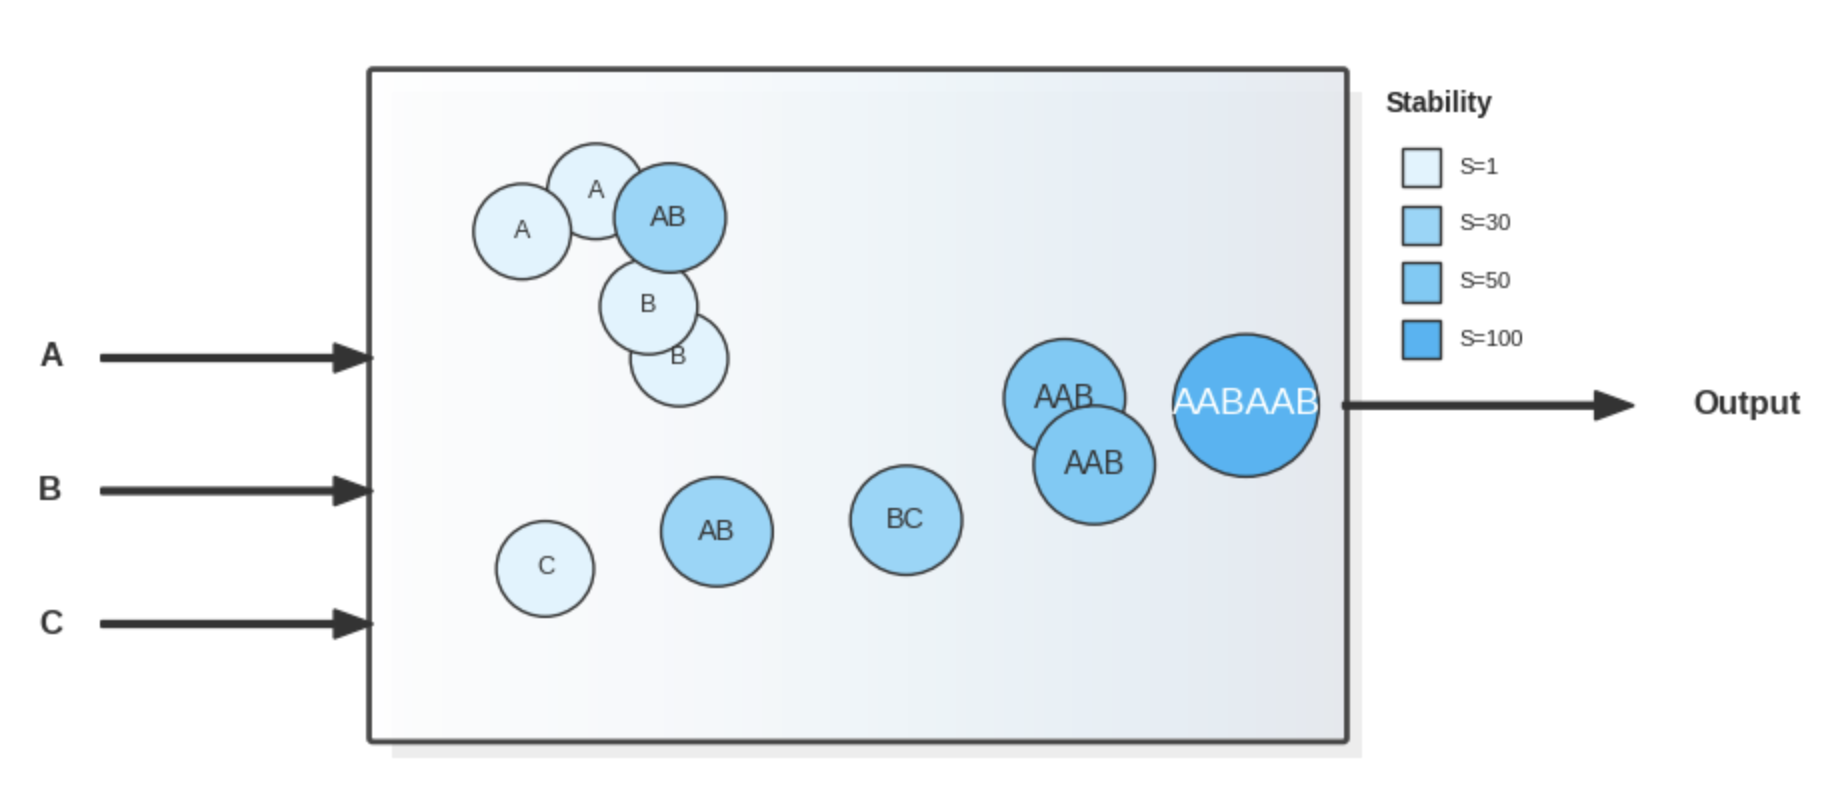
\includegraphics[height=5cm]{figure_1}
    \caption{SDSA analogue of a chemical Continuous Flow Stirred Tank Reactor (CFSTR)}
    \label{fig:figure_1}
\end{figure}

\subsection{Formal Definition}

A Stability-Driven Stochastic Assembly (SDSA) system is formally defined as a tuple $(E, P, S, R, I)$ where:
\begin{itemize}
   \item $E = \{e_1, e_2, \ldots, e_n\}$ is a finite set of base elements
   \item $P$ is the set of all possible patterns formed by concatenating elements from $E$ and existing patterns, with each pattern $p \in P$ being a string over the alphabet $E$
   \item $S: P \rightarrow \mathbb{Z}^{+}$ is a stability function mapping each pattern to a non-negative integer representing its lifetime in generations
   \item $R: E \rightarrow \mathbb{Z}^{+}$ is a replenishment function specifying how many copies of each base element are added per generation
   \item $I \in \mathbb{Z}^{+}$ is the number of interactions allowed per generation
\end{itemize}

The state of the system at generation $t$ is defined by the set of patterns present in the population, with each pattern's presence implicitly determining its probability of selection for interactions. The pattern interaction operation, denoted by $\oplus$, is defined as string concatenation. When patterns $p_1$ and $p_2$ interact, they form pattern $p_1 \oplus p_2$.


\begin{algorithm}[H]
\caption{SDSA System Simulation}
\begin{algorithmic}[1]
\REQUIRE Set of base elements $E$, stability function $S$, replenishment rates $R$, interaction count $I$, generations $T$
\ENSURE Evolution of pattern population over $T$ generations
\STATE Initialize population with base elements according to initial conditions
\FOR{$t = 1$ to $T$}
   \STATE Remove patterns that have reached their stability-determined expiration time
   \FOR{each element $e \in E$}
       \STATE Add $R(e)$ copies of element $e$ to the population
   \ENDFOR
   \FOR{interaction count from $1$ to $I$}
       \STATE Randomly select two patterns from the current population
       \STATE Form new pattern $p_{new}$ by concatenating the selected patterns
       \STATE Determine stability lifetime $S(p_{new})$ for the new pattern
       \STATE Add the new pattern to the population with creation time $t$ and expiration time $t + S(p_{new})$
   \ENDFOR
   \STATE Record population state for analysis (optional)
\ENDFOR
\RETURN Pattern population evolution
\end{algorithmic}
\end{algorithm}


The probability of selecting a pattern $p$ for interaction in generation $t$ is naturally proportional to its frequency in the population. This creates a statistical feedback mechanism: patterns with higher stability persist longer, becoming more abundant in the population, which increases their probability of participating in interactions and forming new compounds.

\subsection{Illustrative Examples}

Consider a simple SDSA system starting with a few instances of the base elements \( A \) and \( B \). The pattern \( AB \) has a lifetime of 10 generations, while \( ABAB \) has a lifetime of 50 generations, and all other compounds degrade instantly with a lifetime of 0. After the first generation, the system produces combinations such as \( AA \), \( BB \), and \( AB \). Since \( AA \) and \( BB \) are unstable, they are eliminated, leaving \( A \), \( B \), and \( AB \). In subsequent generations, new unstable patterns may appear transiently, but \( AB \) persists due to its longer lifetime. The abundance of \( AB \) naturally increases as it persists, raising the probability of forming \( ABAB \). This dynamic reflects a form of roulette wheel selection \cite{goldberg1989genetic} \cite{holland1975adaptation}, where stability-driven persistence affects interaction probability. The emergent pattern \( ABAB \) represents a higher-order configuration, demonstrating how selection, grounded in differential stability, shapes the system's evolutionary pathways. 

The following simulation shows a different SDSA system, with a population of 3 elements: {A, B, C}. Assume that the B compounds are more stable than those without B. Thus, patterns like BB, AB, BC, and ABC have a higher stability than AC, A, or C. Therefore, B compounds will persist for multiple generations, while all others will dissipate. The more stable B-compounds will interact more frequently as a result of their relative frequency, even though there is no replication or inheritance at the individual compound level. A snapshot of the simulation is shown in Figure \ref{fig:figure_2}.

\begin{figure}[htp]
    \centering
    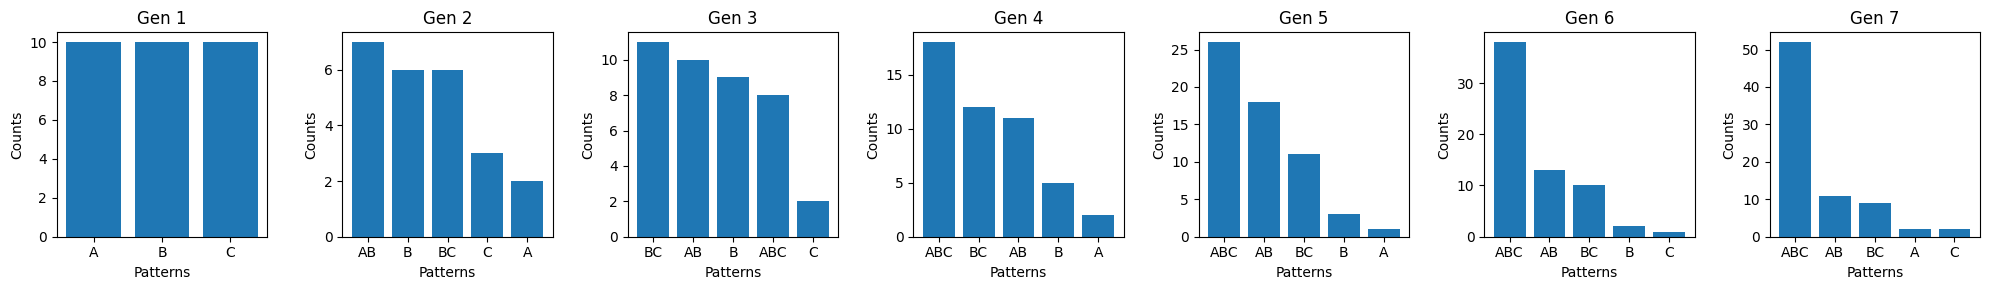
\includegraphics[width=1\textwidth]{figure_2}
    \caption{SDSA System population evolution simulation}
    \label{fig:figure_2}
\end{figure}

Where is Maxwell's demon \cite{leff2002maxwell} hiding in Figure \ref{fig:figure_2}, driving it towards a low-entropy state? As we saw, the answer lies in the roulette wheel. Compounds that persist longer have more chances to interact. As their frequency in the population increases, their chances to interact grow even more. In Evolutionary Dynamics, this is called fitness-proportionate selection \cite{back1996evolutionary} or roulette wheel selection \cite{goldberg1989genetic} \cite{holland1975adaptation}.


\section{Analysis of SDSA Systems Using Probability Distributions}

This section analyzes the behavior of SDSA systems through probability theory, providing a mathematical framework for understanding how stability-driven selection shapes population dynamics over time.

\subsection{Population and Stability Distributions}

We can analyze SDSA systems through two key distributions: the \textbf{population distribution}, which represents the relative abundance of patterns in the system, and the \textbf{stability distribution}, which quantifies pattern lifetimes. The population distribution at generation \( t \) can be defined as \( P_t(p) = \frac{N_t(p)}{\sum_{q \in P} N_t(q)} \), where \( N_t(p) \) is the count of pattern \( p \) at generation \( t \). This distribution evolves over time as patterns with different stabilities interact and persist.

The stability function \( S: P \rightarrow \mathbb{Z}^{+} \) maps each pattern to its lifetime in generations. Unlike the population distribution, which evolves dynamically based on interactions, the stability function is typically defined externally and remains constant throughout the simulation.

In applications to real-world scenarios, the values of \(S(p)\) would be determined by underlying physical, chemical, or other domain-specific principles. For example, in a chemical context, stability values might correspond to binding energies or activation barriers; in an economic model, they could represent market resilience or competitive advantage. The stability function encodes the persistence property that drives selection in SDSA systems.

\subsection{Analytical Model of Pattern Dynamics}

To understand SDSA system evolution analytically, we can model how pattern probabilities change across generations. The probability of observing pattern \(p\) at generation \(t+1\) results from two distinct processes: the persistence of existing copies and the creation of new copies through interactions.

For persistence analysis, we need to account for how pattern instances with different creation times contribute to the population. Given that pattern \(p\) has a deterministic lifetime of \(S(p)\) generations, we can express the persistence component as:

\begin{equation}
\label{eq:persist-term}
\mathrm{Persist}_t(p) = P_t(p) \cdot \left(1 - \frac{1}{\overline{R}_t(p)}\right)
\end{equation}

Where \(\overline{R}_t(p)\) represents the average remaining lifetime of pattern \(p\) instances in the population at generation \(t\), with \(\overline{R}_t(p) \leq S(p)\). This term accounts for the age distribution of existing pattern instances without assuming uniform creation rates.

When the system is far from equilibrium or experiencing rapidly changing dynamics, \(\overline{R}_t(p)\) may vary significantly between generations. In a perfectly stable system with a constant creation rate, \(\overline{R}_t(p)\) would approach \(\frac{S(p)+1}{2}\), the average of remaining lifetimes for uniformly distributed ages.

For creation analysis, we can estimate the probability of forming new copies of pattern \(p\) through concatenations:
\begin{equation}
\label{eq:create-term}
\mathrm{Create}_t(p) = \sum_{(q,r) \to p} P_t(q) \cdot P_t(r)
\end{equation}

Where the notation \((q,r) \to p\) indicates pattern pairs that, when concatenated, form pattern \(p\). For example, pattern ABA can form from AB+A or A+BA.

Combining these processes and normalizing yields an analytical approximation of the expected population distribution at the next generation:
\begin{equation}
\label{eq:full-ba-update}
P_{t+1}(p) = \frac{
  \mathrm{Persist}_t(p) + \mathrm{Create}_t(p)
}{
  \sum_{p' \in P} 
  \left[
    \mathrm{Persist}_t(p') + \mathrm{Create}_t(p')
  \right]
}
\end{equation}

It is important to note that this analytical model approximates the behavior of the SDSA simulation rather than defining it. The actual simulation proceeds according to the algorithm defined earlier, while this model helps us understand and predict the statistical properties of the system.

\subsection{Entropy Dynamics Analysis}

Analysis of Equation~\ref{eq:full-ba-update} reveals two competing processes determining probability shifts across generations:
\begin{equation}
P_{t+1}(p) \propto \mathrm{Persist}_t(p) + \mathrm{Create}_t(p)
\end{equation}

To quantify how stability differences drive entropy reduction, we can analyze the conditions under which the system evolves toward lower-entropy states. The Shannon entropy of the population distribution at time $t$ is given by:
\begin{equation}
H(P_t) = -\sum_{p \in P} P_t(p) \log P_t(p)
\end{equation}

For entropy to decrease over time ($H(P_{t+1}) < H(P_t)$), the population distribution must become more concentrated. This depends critically on the relative magnitudes of pattern stabilities and their distribution.

We can derive a condition for entropy reduction by examining when the persistence advantage of stable patterns outweighs the entropy-increasing effect of random pattern creation. Consider a system with two types of patterns: high-stability patterns with $S(p) = S_{high}$ and low-stability patterns with $S(p) = S_{low}$.

For high-stability patterns to increase their relative frequency in the population (thus reducing entropy), the following condition must hold:

\begin{equation}
\frac{P_t(p_{high}) \cdot (1 - \frac{1}{\overline{R}_t(p_{high})})}{P_t(p_{low}) \cdot (1 - \frac{1}{\overline{R}_t(p_{low})})} > 1
\end{equation}

Assuming that both pattern types have reached their steady-state age distributions where $\overline{R}_t(p) \approx \frac{S(p)+1}{2}$, and simplifying, we get:

\begin{equation}
\frac{S_{high} - 1}{S_{high} + 1} > \frac{S_{low} - 1}{S_{low} + 1}
\end{equation}

This inequality is always satisfied when $S_{high} > S_{low}$, but the magnitude of the difference determines how quickly the distribution will skew. We can define a critical ratio $\rho^*$ that indicates when stability-driven selection will dominate over random creation effects:

\begin{equation}
\rho^* = \frac{S_{high}}{S_{low}} > \frac{|P| \cdot (S_{low} + 1)}{S_{low} - 1}
\end{equation}

Where $|P|$ represents the number of distinct patterns in the population. This threshold captures the critical relationship between stability differences and population diversity. 

For large $S_{low}$ values, this simplifies to $\rho^* \approx |P|$, meaning that for significant entropy reduction, the highest stability should exceed the lowest by approximately a factor equal to the pattern diversity. When this condition is met, the system will evolve toward states dominated by the high-stability patterns, exhibiting substantial entropy reduction.


\section{Mixing Two SDSA Systems}

Mixing two independently evolved Stability-Driven Stochastic Assembly (SDSA) systems introduces a new layer of complexity, where patterns and interactions from each system influence and reshape one another. This interaction results in the exchange of information, changes in entropy dynamics, and the emergence of novel patterns that were inaccessible within isolated systems.

Consider two independently evolved SDSA systems, each representing populations of compounds derived from distinct base elements: \( A, B, C\) for the first system and \( X, Y, Z\) for the second. Each system evolves separately, guided by its population distribution and node stability constraints. Upon mixing, the systems form a joint network in which patterns from both systems interact to create compounds between systems (e.g. \( ABXX, BBYZ \)). Stability constraints, which govern the persistence of patterns, extend to these intersystem interactions, creating a dynamic interplay that determines the joint system's evolution. The updated probabilities in the combined system reflect both the within-system interactions and the newly formed cross-system interactions, as depicted in Figure~\ref{fig:figure_3}.

\begin{figure}[htp]
    \centering
    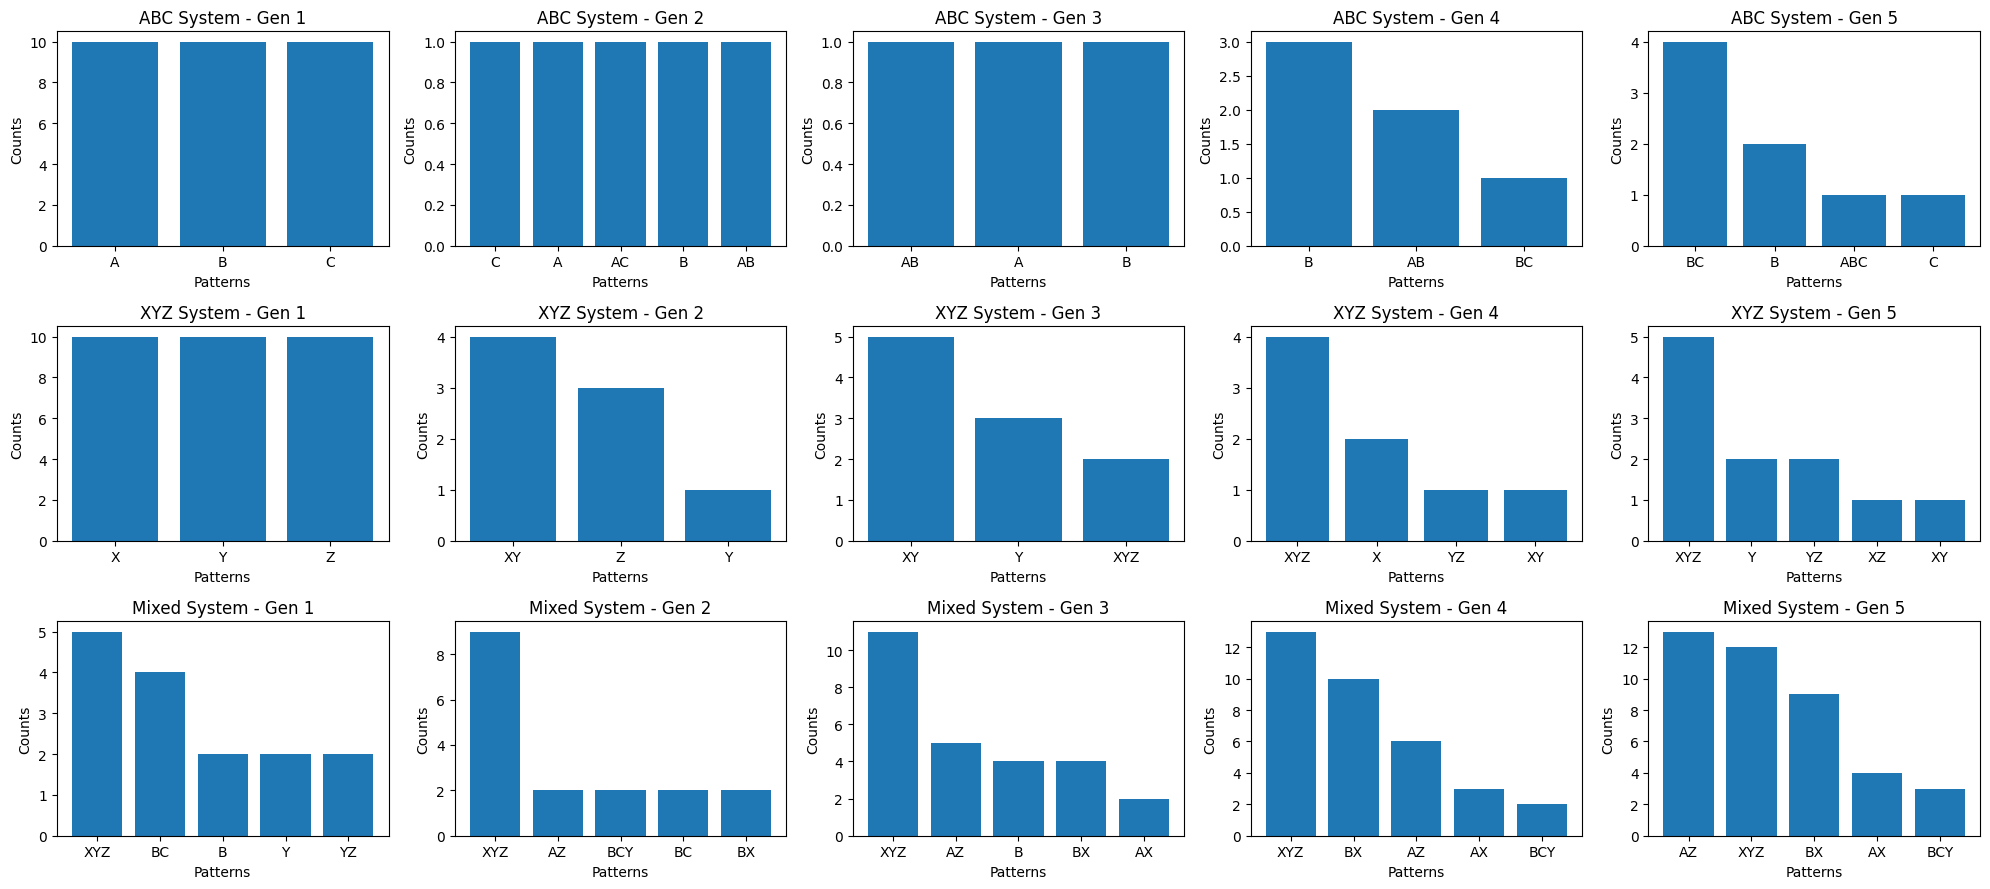
\includegraphics[width=13cm]{figure_3}
    \caption{Mixing two independently evolved populations in a Bayesian Assembly system. Cross-system interactions enable the emergence of novel compounds with high stability, fostering a broader exploration of the state space.}
    \label{fig:figure_3}
\end{figure}

An analogous process occurs in a continuous-flow stirred tank reactor (CFSTR) \cite{fogler1999chemical}, where two distinct chemical feeds are mixed to produce a steady-state mixture. Within this reactor, reactants from each feed can participate in cross-reactions, occasionally generating novel compounds (e.g. \( AZ \)) that exhibit greater stability than those found in either feed alone. 

Mixing two SDSA systems introduces a larger combined stable state space, where the stable patterns that evolved independently within each system now have increased opportunities to cross-interact. New stable cross-products will only form if their stability is higher than existing stable patterns in each population, possibly decreasing the overall entropy.

\section{Why Bayesian Assembly?}

The term Stability-Driven Stochastic Assembly (SDSA) is motivated by the system's iterative updating of probability distributions, analogous to Bayesian inference. In SDSA systems, the probability of each pattern \( P_t(p) \) in generation \( t \) acts as a prior, which is then updated based on stability and interaction dynamics to produce a posterior \( P_{t+1}(p) \) in the next generation. 

We previously saw that $P_{t+1}(p) \propto\ Persist_t(p) + Create_t(p)$, where stability \( S(p) \) plays a role in $Persist(p)$ similar to a Bayesian likelihood function, determining the persistence of existing patterns (which are the observed data). The term $Create(p)$ measures the rate of creation of new copies of patterns, so it does not depend directly on the pattern already existing in the population. Le \cite{le2020equation} has shown that evolutionary processes generally follow a Bayesian update dynamic, where the prior and posterior correspond to the distributions of successive generations. 

The evolving probability distribution in Stability-Driven Stochastic Assembly (SDSA) systems is an elaboration of Kauffman's \emph{Theory of the Adjacent Possible} \cite{kauffman2000investigations, kauffman2024tap}, which describes that new states become accessible as existing structures form but does not propose a selection mechanism. SDSA systems may provide the missing mechanism for the exploration of the "adjacent possible".

\section{Do SDSA Systems Truly Evolve?}

A natural question arises: do SDSA systems genuinely evolve, or is "evolution" merely an analogy? Although SDSA systems lack explicit self-replication at the level of individual instances of a pattern $p_i$, they exhibit population-level dynamics that are mathematically indistinguishable from classical evolutionary processes. 

The fundamental mechanism driving this behavior is that more copies of $p$ are sustainably created from the precursor patterns, leading to an increasing relative abundance $N_p$ in the population. Moreover, the stability function $S(p)$ ensures that higher stability patterns persist longer before being degraded or replaced, further amplifying their representation. 

These dynamics align with the principles of fitness-weighted selection in evolutionary systems, where persistence and reproductive opportunity drive the emergence of dominant patterns. Since the probability of $p$'s continued presence is explicitly governed by its relative abundance and stability, resulting in a roulette wheel selection process, we may assert that SDSA systems exhibit genuine evolutionary behavior, not as a mere analogy, but as a mathematical inevitability.


\section{Simulation of Unconstrained and Bayesian Assembly Systems}

Unconstrained systems allow all possible compounds to form with equal likelihood in each generation, leading to unbounded combinatorial expansion of the state space. If $N_t$ is the total number of compounds present in generation $t$, the probability of observing a specific compound $p$ can be approximated by $P_t(p) = \frac{1}{N_t}$. $N_t$ grows with $t$, so $P_t(p) \to \epsilon$ for any single compound. This uniform dispersion implies that no pattern dominates. The entropy of the system increases as more compounds enter the state space.

To compare the dynamics of unconstrained and SDSA systems, we developed a simulation framework that models the evolution of compound formation over successive generations. This framework captures the key contrasts between the two regimes: the uniform expansion of state space of the unconstrained system and the stability-driven selection pressures of the SDSA system. The simulation begins with an initial population of base elements and proceeds through a fixed number of generations. The following pseudocode captures the main steps and shows that the only difference between the unconstrained and SDSA systems is the setting of expiration times for compounds based on their stability.

\begin{center}
\begin{minipage}{0.9\textwidth}
\ttfamily
\begin{verbatim}
Initialize population with base elements
For each generation:
    Replenish base elements in population
    For each interaction:
        Randomly select a pair of elements from population
        Form compound by concatenation and add to population
        If SDSA system:
            Set compound expiration based on S(p)
    Remove expired elements from population
    Compact patterns into simplified representations
    Store population data for analysis
\end{verbatim}
\end{minipage}
\end{center}
The simulation results in Figure \ref{fig:figure_4} confirm that the unconstrained system disperses its probabilities over an expanding set of compounds, mirroring a uniform exploration of the combinatorial state space with high entropy. In contrast, the SDSA system channels probability into a subset of stable compounds. High-stability patterns become attractors, reducing entropy as the system evolves. Figure~\ref{fig:figure_4} illustrates these differences: while the unconstrained distribution remains broad and diffuse, the SDSA distribution skews heavily toward stable patterns and a peaked distribution which reduces entropy.

\begin{figure}[h]
    \centering
    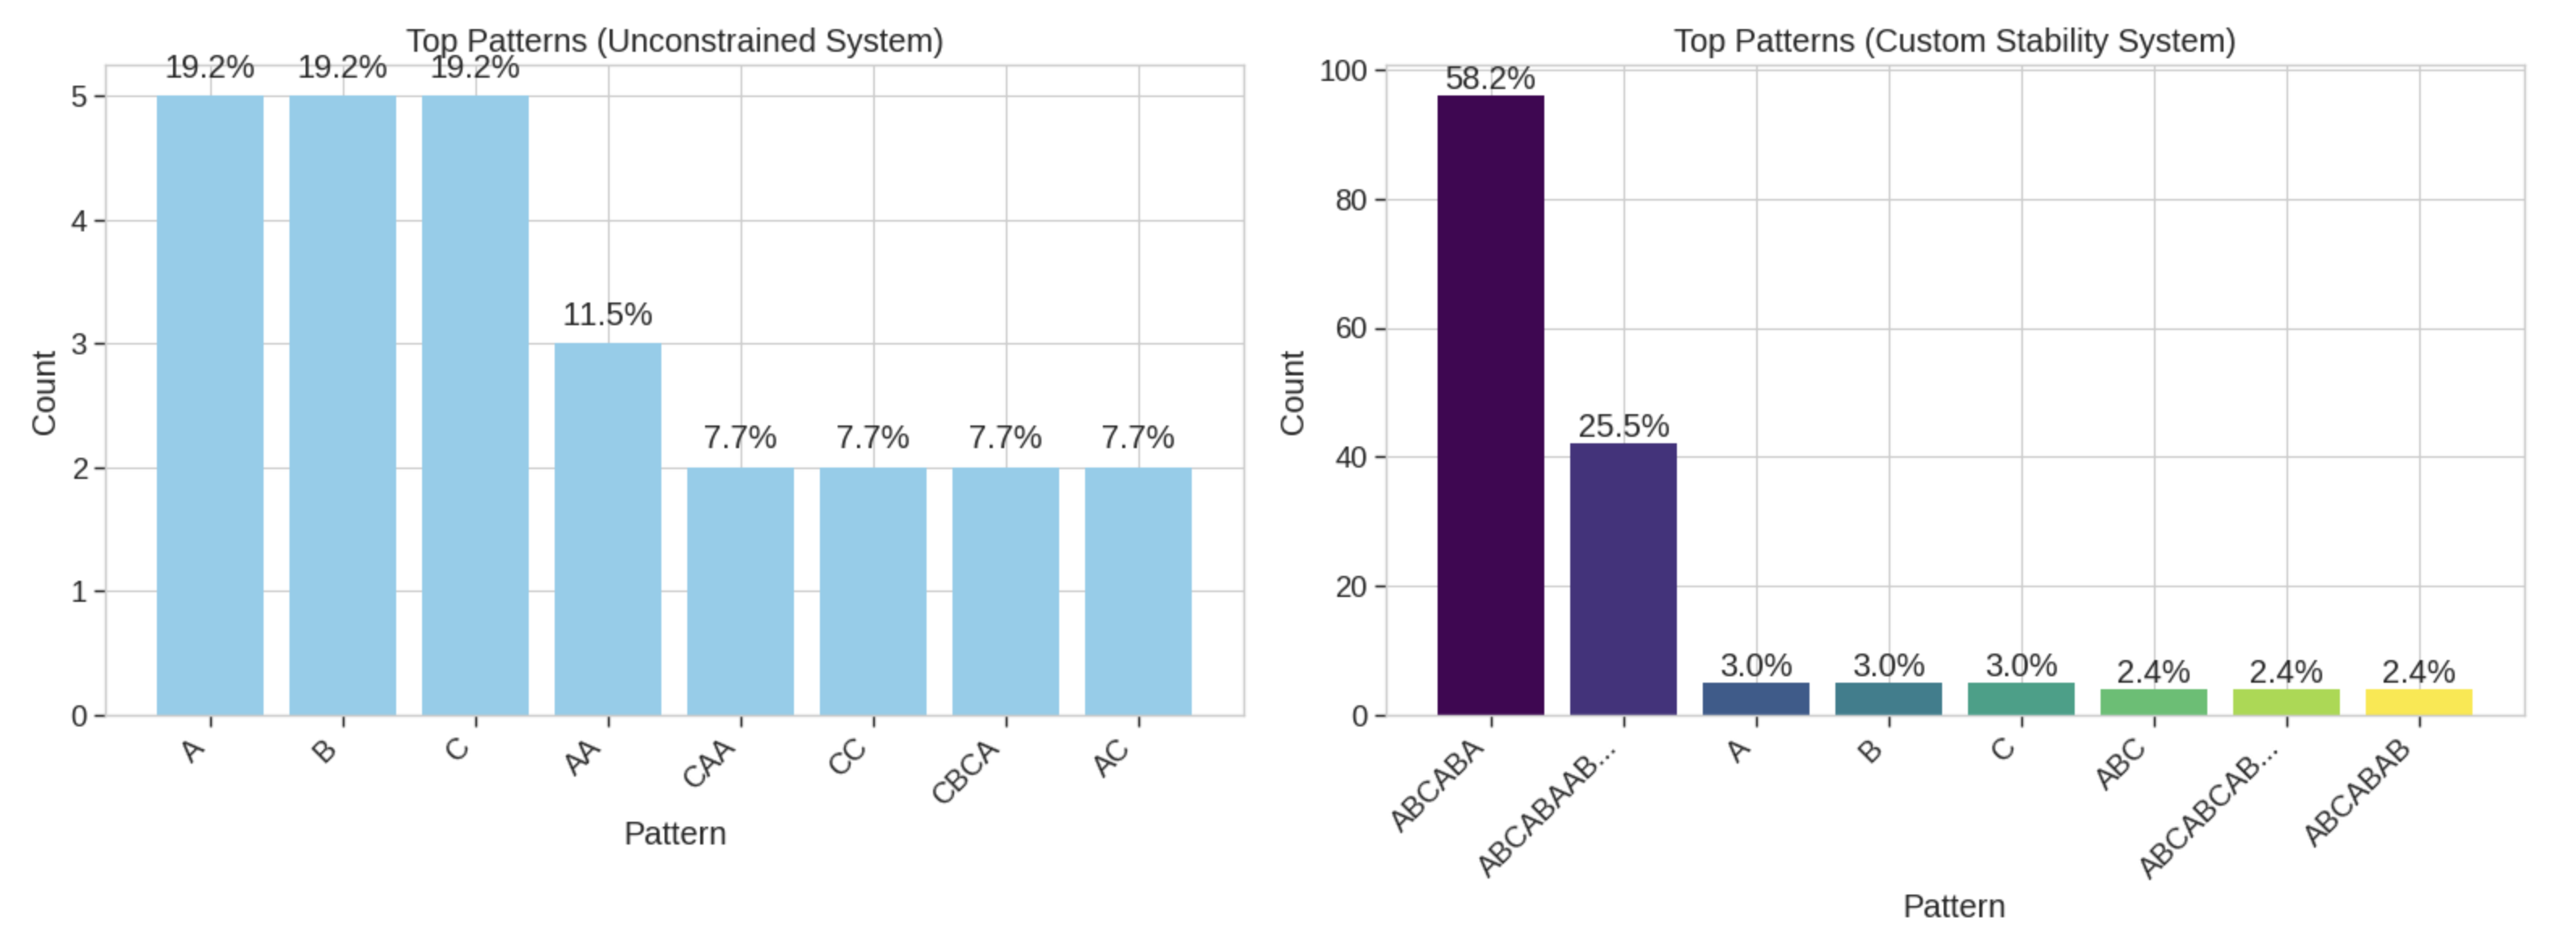
\includegraphics[width=1\textwidth,height=6cm]{figure_4.png}
    \caption{Simulation of  unconstrained system (uniform distribution) and SDSA systems (peaked distribution).}
    \label{fig:figure_4}
 \end{figure}

\section{Dynamic Graph Representation and Token Flow Analysis}

To further investigate the dynamics of SDSA systems, we represent the state of the system in a specific generation as a directed graph, where the nodes correspond to base elements and compounds such as $A$, $AB$, $ABA$, $ABC$, and the directed edges represent the interactions that occurred between them in their assembly process. The base elements $A$, $B$, $C$ are replenished in each generation, initiating a cascade of interactions that propagate tokens (shown in Figure~\ref{fig:figure_5} as the count $N$ of instances or copies of each pattern). 

The token flow describes the redistribution of these tokens between nodes in the reaction graph, driven by stability dynamics and interactions. This process is analogous to probability currents in quantum mechanics \cite{feynman1965quantum} and optimal transport \cite{villani2008optimal}, reflecting the macroscopic evolution of the system. The tokens accumulate at nodes based on the flow dynamics, which are governed by the stability of each pattern (shown in Figure~\ref{fig:figure_5} as $S$), influencing the persistence and selection of patterns over successive generations.


\begin{figure}[h]
    \centering
    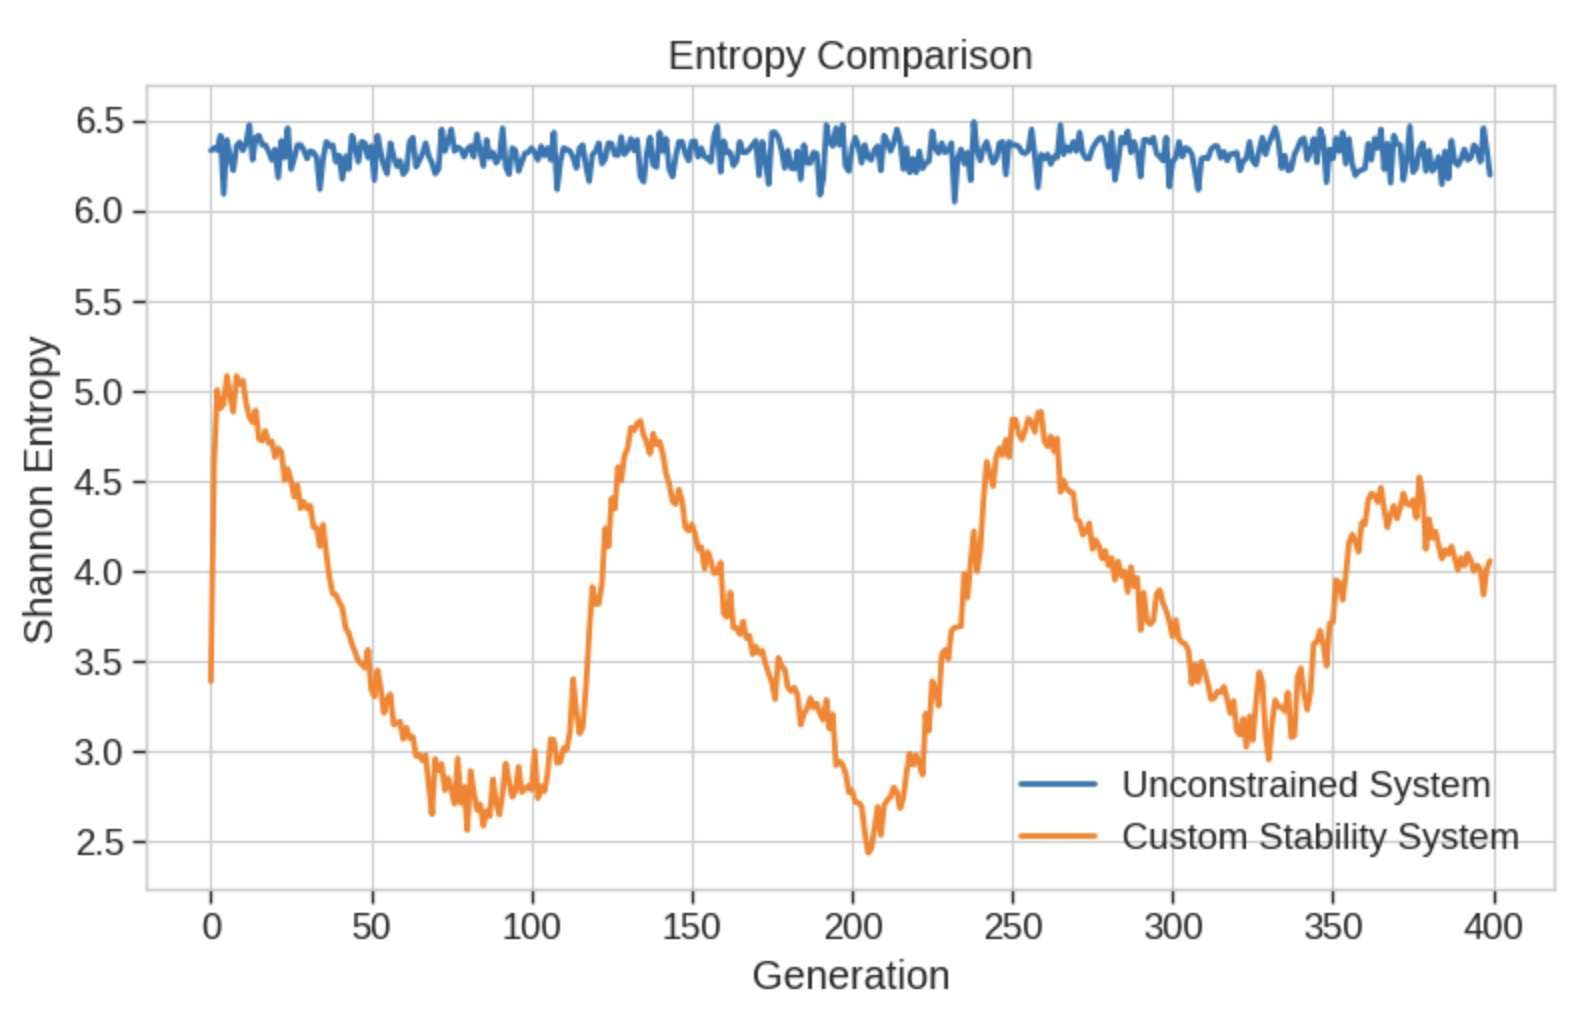
\includegraphics[width=0.7\linewidth]{figure_5.png}
    \caption{Graph representation of a SDSA system showing stability (S), and the number of instances or tokens (N) of each base element and compound.}
    \label{fig:figure_5}
\end{figure}

The dynamic graph in Figure~\ref{fig:figure_5} represents the 7th generation of the simulation shown in Figure~\ref{fig:figure_4}. The distribution of tokens across the graph reveals insights into the self-reinforcing nature of stability in SDSA systems. Nodes with higher stability values (\textit{ e.g.}, $ABCABA$) attract more tokens, leading to the emergence of dominant patterns. This phenomenon reflects a feedback loop: As tokens accumulate at a stable node, it becomes increasingly likely to dominate subsequent interactions, establishing preferential flow paths through the graph. Consequently, the system's token traffic converges to well-defined routes, concentrating resources on a subset of high-stability patterns while marginalizing less stable ones.

However, the graph may change significantly between generations if a new disruptor node emerges in the system. A disruptor node is characterized by a high stability value and strategic positioning within the graph, enabling it to compete with previously dominant nodes for token traffic. This disruptor can reroute flows, effectively redistributing tokens and breaking established dominance patterns. The behavior of token flows in the SDSA system parallels physical phenomena, such as those observed in fluid systems, where a new high-conductivity channel can divert flow away from existing pathways. Similarly, in RC circuits, the introduction of a new low-resistance branch redistributes the current, altering the overall system equilibrium. 

Dynamic graphs have been used for switch-level simulation of transistor networks \cite{AdlerCAD}, where graph pathways are dynamically determined by the state of the on transistors, enabling specific connections to guide current flow. Similarly, in SDSA systems, token flow is governed by stability and probabilistic interactions, determining which nodes persist and propagate.

\section{Chemical Example: Iron Oxidation}

\begin{figure}[h]
    \centering
    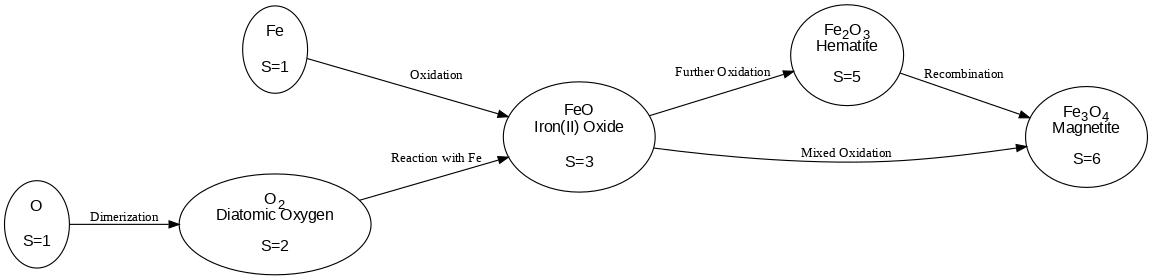
\includegraphics[width=1\textwidth,height=0.4\textwidth]{figure_6.png}
    \caption{Reaction network for iron oxidation, illustrating the stepwise formation of stable and intermediate compounds under stability constraints.}
    \label{fig:figure_6}
\end{figure}

The principles of Stability-Driven Stochastic Assembly (SDSA) systems can be illustrated through the oxidation of iron, a realistic and naturally occurring chemical process. As shown in Figure~\ref{fig:figure_6}, iron oxidation (\(Fe\)) proceeds through a network of reactions driven by stability constraints. Oxygen (\(O\)) forms diatomic oxygen (\(O_2\)), which reacts with iron to produce a series of oxides, including iron(II) oxide (\(FeO\)), iron(III) oxide (\(Fe_2O_3\), hematite), and iron(II,III) oxide (\(Fe_3O_4\), magnetite). These reactions represent a progression from less stable intermediates to thermodynamically favored compounds. Competing pathways, such as partial oxidation or the formation of unstable intermediates, illustrate how stability shapes the evolution of the system, favoring reactions that lead to more persistent and energetically favorable products.

In the SDSA framework, node stability \(S(p)\) quantifies the persistence of each compound, with higher stability values assigned to products such as hematite and magnetite due to their robust bonding and lower susceptibility to dissociation. This reaction network provides a testable system for validating the role of stability in driving reaction pathways. By simulating token flow dynamics based on stability values, the framework captures how high-stability compounds emerge and dominate over successive generations, aligning with experimental observations of oxidation processes.




\section{Economic Example: Industry Ecosystem as a SDSA System}

This example illustrates a Stability-Driven Stochastic Assembly (SDSA) system applied to an economic context, where base elements represent different types of businesses. Manufacturers (A), retailers (B), and logistics providers (C) act as base elements with stabilities \( S_A, S_B, S_C \) reflecting their persistence in the market. Through successive interactions, these base elements form partnerships \( AB \), \( AC \), \( BC \) and evolve into integrated networks \( ABAC \), \( ABBC \), as shown in Figure~\ref{fig:figure_9}. Each stage corresponds to increasingly complex collaborations, where stability-driven selection ensures the persistence of dominant nodes. 

\begin{figure}[h]
    \centering
    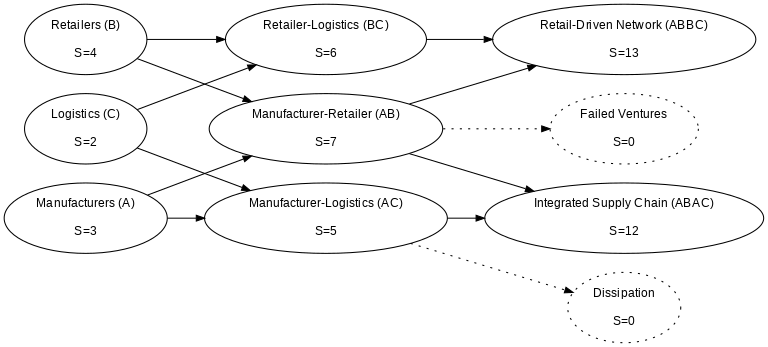
\includegraphics[width=1\textwidth]{figure_9.png}
    \caption{Industry ecosystem represented as a SDSA system, showing the evolution from base businesses (\( A, B, C \)) to partnerships and stable integrated networks (\( ABAC, ABBC \)).}
    \label{fig:figure_9}
\end{figure}

Stable nodes, such as \( AB \) (manufacturer-retailer) and \( ABBC \) (retail-driven networks), act as attractors, accumulating resources (tokens) over generations. Less stable nodes, including failed ventures (\( S=0 \)), dissipate quickly, redistributing tokens to more viable configurations. The economic analogy emphasizes how stability influences token flow, resource allocation, and the formation of hierarchical networks in complex systems. The tokens in this graph (individual companies) will naturally flow to configurations that are more stable and persistent, representing more business opportunities.

\section{Top-Down vs.\ Bottom-Up Dynamics in SDSA Systems}
\label{sec:topdown-bottomup}

Figure~\ref{fig:figure_10} illustrates the interplay between top-down and bottom-up causation in Stability-Driven Stochastic Assembly (SDSA) systems, where the top-down influence emerges from the increasing relative abundance of stable patterns directing subsequent interactions, while bottom-up processes arise from the probabilistic assembly of base elements into intermediate and complex patterns, creating a dynamic feedback loop that drives the evolution of information and complexity.

\begin{figure}[h]
    \centering
    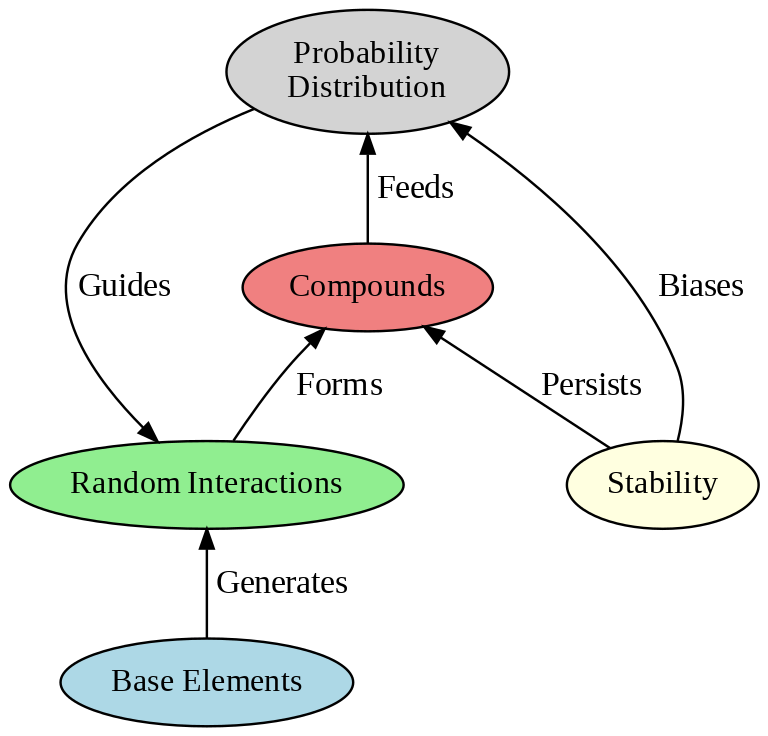
\includegraphics[width=0.7\linewidth,height=0.7\linewidth]{figure_10.png}
    \caption{Bottom-up and Top-down causation in SDSA systems}
    \label{fig:figure_10}
\end{figure}

Once certain patterns become dominant, they exert a top-down influence on subsequent generations. These higher-level persistent structures shape future interactions by catalyzing or constraining the formation of new patterns. Hence, SDSA systems do not just accumulate complexity through local rules; they also incorporate feedback from emergent structures that guide (or ``select for'') new configurations. The presence of memory and evolutionary history in these feedback loops distinguishes SDSA systems from frameworks in which higher-level states simply describe aggregates without influencing the underlying microstates.

The contrast with traditional statistical mechanics is instructive \cite{landau1980statistical}. In statistical mechanics, macrostates (e.g., temperature, pressure) represent aggregate properties of microstates but do not directly influence the fundamental interaction rules among particles. In SDSA systems, however, dominant patterns exert a causal influence on micro-level interactions, embedding history and specificity into the generative process itself. This dynamic distinguishes SDSA systems by allowing feedback mechanisms that shape pattern evolution, separate from physical energy distributions or equilibrium constraints.

Such an explicit interplay between bottom-up and top-down dynamics in SDSA systems suggests a broader principle for understanding complexity: emergent structures can become causal agents that direct further evolution of the system. This perspective helps explain the accumulation of novel order in contexts ranging from prebiotic chemistry to computational networks, where higher-level assemblies (compounds, motifs, or functional components) increasingly govern local interactions, thereby catalyzing the exploration of new possibilities for growth and adaptation.

At times, these dynamics appear teleological, as if the system were ``seeking'' more stable or more complex configurations. Bertalanffy \cite{bertalanffy1968general} cautions that such optimization processes, while suggestive of goal-directed behavior, often reflect nothing more than the natural unfolding of selection, feedback loops, and probability gradients rather than true purposeful design. SDSA systems likewise illustrate how feedback from emergent structures can drive the exploration of new system states without implying an external or predetermined goal. By capturing both bottom-up and top-down mechanisms in an evolving distribution, SDSA systems provide a model for understanding how complexity can accumulate, whether in prebiotic chemistry or in computational and informational domains, through iterative processes of selection and the continual reshaping of local interactions.


\section{Conclusion}

SDSA systems provide a simple framework for understanding the emergence of complexity and order in systems governed by probabilistic interactions and stability-driven selection. By abstracting away specific physical laws, these systems offer a testable and generalizable model applicable to a wide range of phenomena. 

The iterative interaction of elements in SDSA systems may help explain the evolution of matter and energy. From the aggregation of quarks into elementary particles, to the evolution of molecules and chemistry. The periodic table, for example, organizes elements based on properties such as ionization energy, chemical reactivity, etc. These properties bias element interactions, favoring stable configurations. For example, \( H_2 \) forms in dense regions of space where hydrogen atoms collide and bond. It is stable because of strong covalent bonds and serves as a building block for stars. This reflects the dominance of stability-driven patterns, akin to how SDSA systems reinforce stable patterns over generations. 

SDSA systems suggest that evolution may be a universal property of random populations with large stability imbalances, not restricted to living organisms. By demonstrating how random populations with stability-driven interactions naturally evolve toward order, this framework proposes that perhaps the biological evolution of individual organisms is a later stage in such dynamics. Recent findings suggest that stability-driven self-assembly mechanisms may play a role in biotic systems, highlighting the possible connection between abiotic and biological evolution \cite{davies2022selfassembly}.

SDSA systems may provide a non-mystical explanation of the origins of order and information. Unlike Tegmark's \cite{tegmark2008mathematical} assertion that physical reality is a purely mathematical structure, or Wolfram's \cite{wolfram2020fundamental} derivation of physical laws from abstract cellular automata, SDSA systems remain firmly within observable, probabilistic mechanisms of selection. Similarly, while Bohm's ontological interpretation of quantum mechanics \cite{bohm1980wholeness} proposes an implicate order from which observable reality unfolds as a mystical pilot wave, SDSA systems focus on generational updates grounded in explicit and testable mechanisms of interaction and population dynamics.

SDSA systems still leave open the question of fine-tuning. Fine-tuned imbalances, such as those described in Rees' \textit{Just Six Numbers} \cite{rees2000just} and Davies' \textit{The Goldilocks Enigma} \cite{davies2006goldilocks}, exemplify how asymmetries in fundamental physical constants enable complexity across scales. Similarly, in SDSA systems,  non-uniform stability biases interactions toward forming persistent ordered patterns. This connection reinforces the idea that evolution, driven by imbalance and selection, operates universally, bridging the emergence of complexity from the cosmological to molecular scales. If further empirical evidence shows that large stability imbalances play a key role in the evolution of the universe, then one might be tempted to say that God does indeed play dice, but the dice are loaded.


%\begin{listing}[H]
%\caption{Title of the listing}
%\rule{\columnwidth}{1pt}
%\raggedright Text of the listing. In font size footnotesize, small, or normalsize. Preferred format: left aligned and single spaced. Preferred border format: top border line and bottom border line.
%\rule{\columnwidth}{1pt}
%\end{listing}

%%%%%%%%%%%%%%%%%%%%%%%%%%%%%%%%%%%%%%%%%%
\vspace{6pt} 

%%%%%%%%%%%%%%%%%%%%%%%%%%%%%%%%%%%%%%%%%%
%% optional
%\supplementary{The following supporting information can be downloaded at:  \linksupplementary{s1}, Figure S1: title; Table S1: title; Video S1: title.}

% Only for journal Methods and Protocols:
% If you wish to submit a video article, please do so with any other supplementary material.
% \supplementary{The following supporting information can be downloaded at: \linksupplementary{s1}, Figure S1: title; Table S1: title; Video S1: title. A supporting video article is available at doi: link.}

% Only for journal Hardware:
% If you wish to submit a video article, please do so with any other supplementary material.
% \supplementary{The following supporting information can be downloaded at: \linksupplementary{s1}, Figure S1: title; Table S1: title; Video S1: title.\vspace{6pt}\\
%\begin{tabularx}{\textwidth}{lll}
%\toprule
%\textbf{Name} & \textbf{Type} & \textbf{Description} \\
%\midrule
%S1 & Python script (.py) & Script of python source code used in XX \\
%S2 & Text (.txt) & Script of modelling code used to make Figure X \\
%S3 & Text (.txt) & Raw data from experiment X \\
%S4 & Video (.mp4) & Video demonstrating the hardware in use \\
%... & ... & ... \\
%\bottomrule
%\end{tabularx}
%}

%%%%%%%%%%%%%%%%%%%%%%%%%%%%%%%%%%%%%%%%%%

%\funding{This research received no external funding}

%\institutionalreview{Not applicable}

%\informedconsent{Not applicable}

%\dataavailability{Not applicable} 

%\acknowledgments{}

%\conflictsofinterest{The author declares no conflicts of interest} 

%%%%%%%%%%%%%%%%%%%%%%%%%%%%%%%%%%%%%%%%%%
%%%%%%%%%%%%%%%%%%%%%%%%%%%%%%%%%%%%%%%%%%
%%%%%%%%%%%%%%%%%%%%%%%%%%%%%%%%%%%%%%%%%%
%\printendnotes[custom] % Un-comment to print a list of endnotes

% Please provide either the correct journal abbreviation (e.g. according to the “List of Title Word Abbreviations” http://www.issn.org/services/online-services/access-to-the-ltwa/) or the full name of the journal.
% Citations and References in Supplementary files are permitted provided that they also appear in the reference list here. 

%=====================================
% References, variant A: external bibliography
%=====================================
%\bibliography{your_external_BibTeX_file}

%=====================================
% References, variant B: internal bibliography
%=====================================
\begin{thebibliography}{999}

\bibitem{fontana1991algorithmic}
Fontana, W. Algorithmic chemistry. \textit{Artificial life II} \textbf{1991}, \textit{11}, 159–209.

\bibitem{gillespie2005stochastic}
Gillespie, D. T. Stochastic simulation of chemical kinetics. \textit{Annual review of physical chemistry} \textbf{2007}, \textit{58}, 35–55.

\bibitem{kauffman1986autocatalytic}
Kauffman, S. A. Autocatalytic sets of proteins. \textit{Journal of theoretical biology} \textbf{1986}, \textit{119}, 1–24.

\bibitem{hordijk2011required}
Hordijk, W.; Kauffman, S. A.; Steel, M. Required levels of catalysis for emergence of autocatalytic sets in models of chemical reaction systems. \textit{International journal of molecular sciences} \textbf{2011}, \textit{12}, 3085–3101.

\bibitem{barabasi1999emergence}
Barabási, A.-L.; Albert, R. Emergence of scaling in random networks. \textit{Science} \textbf{1999}, \textit{286}, 509–512.

\bibitem{kauffman1995home}
Kauffman, S. \textit{At Home in the Universe: The Search for the Laws of Self-Organization and Complexity}; Oxford University Press: New York, NY, USA, 1995.

\bibitem{dorogovtsev2000evolution}
Dorogovtsev, S. N.; Mendes, J. F. F. Evolution of networks with aging of sites. \textit{Physical Review E} \textbf{2000}, \textit{62}, 1842–1845.

%ref 1
\bibitem{schrodinger1944life}
Schrödinger, E. \textit{What is Life?}; Cambridge University Press: Cambridge, UK, 1944.

%ref 2
\bibitem{tegmark2008mathematical}
Tegmark, M. The Mathematical Universe. \textit{Found. Phys.} \textbf{2008}, \textit{38}, 101–150. 

%ref 3
\bibitem{fisher1930genetical}
Fisher, R.A. \textit{The Genetical Theory of Natural Selection}; Oxford University Press: Oxford, UK, 1930.

%ref 4
\bibitem{nowak2006evolutionary}
Nowak, M.A. \textit{Evolutionary Dynamics: Exploring the Equations of Life}; Belknap Press: Cambridge, MA, USA, 2006.

%ref 5
\bibitem{wheeler1990itbit}
Wheeler, J.A. Information, Physics, Quantum: The Search for Links. In \textit{Complexity, Entropy, and the Physics of Information}; Zurek, W.H., Ed.; Addison-Wesley: Redwood City, CA, USA, 1990; pp. 3–28.

%ref 6
\bibitem{noble2012causality}
Noble, D. A Theory of Biological Relativity: No Privileged Level of Causation. \textit{Interface Focus} \textbf{2012}, \textit{2}, 55–64.

%ref 7
\bibitem{lloyd2006programming}
Lloyd, S. \textit{Programming the Universe: A Quantum Computer Scientist Takes on the Cosmos}; Alfred A. Knopf: New York, NY, USA, 2006.

%ref 8
\bibitem{kolmogorov1965complexity}
Kolmogorov, A.N. Three Approaches to the Quantitative Definition of Information. \textit{Problemy Peredachi Informatsii} \textbf{1965}, \textit{1}, 3–11.

%ref 9
\bibitem{chaitin1977algorithmic}
Chaitin, G.J. Algorithmic Information Theory. \textit{IBM J. Res. Dev.} \textbf{1977}, \textit{21}, 350–359. 

%ref 10
\bibitem{solomonoff1964formal}
Solomonoff, R.J. A Formal Theory of Inductive Inference. Part I and Part II. \textit{Inf. Control} \textbf{1964}, \textit{7}, 1–22, 224–254.

%ref 11
\bibitem{shannon1948mathematical}
Shannon, C.E. A Mathematical Theory of Communication. \textit{Bell Syst. Tech. J.} \textbf{1948}, \textit{27}, 379–423.

%ref 12
\bibitem{deutsch2013constructor}
Deutsch, D.; Marletto, C. Constructor theory of information. \textit{Proceedings of the Royal Society A: Mathematical, Physical and Engineering Sciences} \textbf{2015}, \textit{471}, 20140540. 

\bibitem{walker2023nature}
S. I. Walker, L. Cronin, and others,
"Assembly theory explains and quantifies selection and evolution across physical and biological systems," \textit{Nature}, \textbf{618}, 619-628 (2023), doi:10.1038/s41586-023-06600-9.

\bibitem{kauffman2024tap}
M. Cortês and S.A. Kauffman and A.R. Liddle and L. Smolin (2024), "The TAP equation: evaluating combinatorial innovation in Biocosmology" arXiv:2204.14115


\bibitem{TuranyiTomlin2014}
Turányi, T., Tomlin, A. S. (2014). \textit{Analysis of Kinetic Reaction Mechanisms}. Springer. doi:10.1007/978-3-642-38516-1.

\bibitem{feinberg1987chemical}
Feinberg, M. (1987). Chemical Reaction Network Structure and the Stability of Complex Isothermal Reactors—I. The Deficiency Zero and Deficiency One Theorems. \textit{Chemical Engineering Science}, 42(10), 2229–2268. doi:10.1016/0009-2509(87)80099-4.

\bibitem{arxiv:q-bio0501016}
Gillespie, D. T. (2005). Stochastic Simulation of Chemical Kinetics. \textit{arXiv:q-bio/0501016}. Retrieved from https://arxiv.org/pdf/q-bio/0501016.

\bibitem{tononi2008phi}
Tononi, G. (2008). Consciousness as Integrated Information: A Provisional Manifesto. \textit{Biological Bulletin}, 215(3), 216–242. doi:10.2307/25470707.

\bibitem{fogler1999chemical}
Fogler, H. S. (1999). \textit{Elements of Chemical Reaction Engineering} (3rd ed.). Prentice Hall.

%ref 13
\bibitem{leff2002maxwell}
Leff, H.S.; Rex, A.F. \textit{Maxwell’s Demon: Entropy, Information, Computing}; Princeton University Press: Princeton, NJ, USA, 2002.

\bibitem{petri1962communication} C. A. Petri, \textit{Communication with Automata}, Technical Report RADC-TR-65-377, Rome Air Development Center, New York, 1966.

%ref 14
\bibitem{back1996evolutionary}
Bäck, T.; Fogel, D.B.; Michalewicz, Z. \textit{Evolutionary Computation 1: Basic Algorithms and Operators}; CRC Press: FL, USA, 2000.

%ref 15
\bibitem{goldberg1989genetic}
Goldberg, D.E. \textit{Genetic Algorithms in Search, Optimization, and Machine Learning}; Addison-Wesley: Boston, MA, USA, 1989.

%ref 16
\bibitem{holland1975adaptation}
Holland, J.H. \textit{Adaptation in Natural and Artificial Systems}; University of Michigan Press: Ann Arbor, MI, USA, 1975.

%ref 20
\bibitem{mcgrayne2011theory}
McGrayne, S.B. \textit{The Theory That Would Not Die: How Bayes' Rule Cracked the Enigma Code, Hunted Down Russian Submarines, and Emerged Triumphant from Two Centuries of Controversy}; Yale University Press: New Haven, CT, USA, 2011.

%ref 21
\bibitem{kauffman2000investigations}
Kauffman, S. \textit{Investigations}; Oxford University Press: New York, NY, USA, 2000.

\bibitem{le2020equation} N. Le, \textit{The Equation of Knowledge: From Bayes’ Rule to a Unified Philosophy of Science}, Philosophical Press, New York, NY, 2020.

\bibitem{DittrichFenizio2005}
P.~Dittrich and P.~S.~di Fenizio, ``Chemical organization theory: towards a theory of constructive dynamical systems,'' \emph{arXiv preprint arXiv:q-bio/0501016}, 2005.


\bibitem{SpiceRef}
L.~W.~Nagel and D.~O.~Pederson, ``SPICE (Simulation Program with Integrated Circuit Emphasis),'' 
{\em University of California, Berkeley}, Memorandum No. ERL-M382, Apr. 1973.

\bibitem{feynman1965quantum}
Feynman, R. P., \& Hibbs, A. R. (1965). \textit{Quantum Mechanics and Path Integrals}. McGraw-Hill.

\bibitem{villani2008optimal}
Villani, C. (2008). \textit{Optimal Transport: Old and New}. Springer Science \& Business Media.


\bibitem{AdlerCAD} D.~Adler, ``Switch Level Simulation Using Dynamic Graph Algorithms,''
{\em IEEE Transactions on Computer-Aided Design of Integrated Circuits and Systems}, vol.~10, March~1991.

\bibitem{FeynmanComp}
R.~P.~Feynman, {\em Feynman Lectures On Computation}, Westview Press, 1996.

%ref 22
\bibitem{landau1980statistical}
Landau, L. D., Lifshitz, E. M. \textit{Statistical Physics}; Pergamon Press, 1980.

%ref 23
\bibitem{bertalanffy1968general}
Bertalanffy, L. von. (1968). \textit{General System Theory}. New York: George Braziller.

%ref 25
\bibitem{davies2022selfassembly}
Davies, J.; Levin, M. Self-Assembly: Synthetic morphology with agential materials. \textit{Nature Reviews Bioengineering} v 1 (2023).

\bibitem{wolfram2020fundamental} S. Wolfram, \textit{A Project to Find the Fundamental Theory of Physics} (Wolfram Media, 2020).

\bibitem{bohm1980wholeness}
D. Bohm and B. J. Hiley, \emph{The Undivided Universe: An Ontological Interpretation of Quantum Theory}, Routledge, London, 1993. ISBN: 978-0415065887.

%ref 26
\bibitem{rees2000just}
Rees, M. \textit{Just Six Numbers: The Deep Forces that Shape the Universe}; Basic Books: New York, NY, USA, 2000.

%ref 27
\bibitem{davies2006goldilocks}
Davies, P. \textit{The Goldilocks Enigma: Why is the Universe Just Right for Life?}; Allen Lane: London, UK, 2006.


\end{thebibliography}

%% Add \usepackage{lineno} before \begin{document} and uncomment 
%% following line to enable line numbers
%% \linenumbers

\appendix

\section{Stability Imbalances in Nature}

The abstract SDSA model is motivated by the vast stability disparities of the universe, from fleeting nuclear states to gravitationally bound structures that last billions of years. These variations in binding energy, environmental interactions, and system resilience may dictate the formation and persistence of low-entropy structures, from molecular networks to planetary systems. Covalent bonds gain longevity in extended lattices such as diamond and graphene, while geological formations evolve over millions of years under pressure and erosion. On cosmological scales, gravitationally bound systems, including planetary and galactic structures, persist across epochs, underscoring the fundamental role of stability in natural organization.

Beyond simple bond strength, the persistence of structures is influenced by factors such as spatial arrangements, catalytic reinforcement, feedback loops, and hierarchical assembly. Biological molecules, for instance, often derive stability not merely from strong covalent bonds but also from folded conformations, cooperative interactions, and self-repair mechanisms. Similarly, geological formations maintain their integrity over deep time due to self-reinforcing stress distributions and dynamic equilibrium with their environment. Table~\ref{tab:binding-forces} summarizes a wider range of stability-driven phenomena, highlighting their characteristic strengths and lifetimes on multiple scales.


\begin{table}
\centering
\caption{Representative Stability Mechanisms in Nature and Their Typical Lifetimes.}
\label{tab:binding-forces}
\begin{tabular}{l l}
\toprule
\textbf{Mechanism} & \textbf{Typical Lifetime} \\
\midrule
Weak Nuclear (Beta Decay) & $\mu$s to minutes \\
Strong Nuclear (Stable Nuclei) & Millions to trillions of years \\
Covalent Bonds (Organic Molecules) & Seconds to billions of years \\
Hydrogen Bonding (DNA, Proteins) & Picoseconds to seconds \\
Ionic Bonds (Salts, Minerals) & Seconds to millennia \\
Geological Structures (Mountains) & Thousands to billions of years \\
Gravitational Systems (Planets, Stars) & Millions to billions of years \\
\bottomrule
\end{tabular}
\end{table}

Table \ref{tab:binding-forces} illustrates how stability is not solely a function of bond strength but arises from evolved hierarchical structures, environmental effects, and self-reinforcing dynamics. In a SDSA system, high-stability patterns accumulate over generations, biasing the reaction landscape towards configurations that persist. This provides a simplified conceptual model for understanding how long-lived low-entropy structures emerge in nature through differential stability selection, whether in chemical systems, geological formations, or cosmic architecture.


\section{Mass Action Kinetics and SDSA Systems}
\label{subsec:mak-forward-limitations}

Mass Action Kinetics (MAK) \cite{TuranyiTomlin2014} provides deterministic rate equations for chemical reactions, such as
\[
\frac{d[A]}{dt} \;=\; -\,k\, [A]\,[B],
\]
where $[A]$ and $[B]$ represent concentrations and $k$ is a rate constant. These equations capture conservation laws for mass and energy and can reflect selection processes under certain conditions. More recent work such as Chemical Organization Theory (COT) \cite{DittrichFenizio2005} emphasizes the finding of closed and self-maintaining collections of species in a fixed reaction network. Assembly Theory (AT) has proposed the use of MAK-like forward models to link object production to assembly indices and copy numbers \cite{walker2023nature}.

MAK inherently allows reactions to run both forward and backward with fixed-rate laws, posing a challenge for assembly frameworks like AT and SDSA that emphasize net forward construction. Although MAK excels at describing known reaction networks under equilibrium or near-equilibrium assumptions, it lacks a mechanism for the open discovery of novel compounds central to BA’s approach.

\subsection{Analogy to Electronic Circuit Simulations}
\label{subsec:spice-analogy}

In MAK models, species concentrations evolve as
$\dot{\mathbf{x}} = \mathbf{A}\,\mathbf{x} + \mathbf{b}$, where \(\mathbf{x}\) represents species concentrations, \(\mathbf{A}\) encodes stoichiometric and kinetic rate constants, and \(\mathbf{b}\) accounts for base element replenishment, driving the system away from thermodynamic equilibrium. A similar formulation appears in electronic circuit simulation \cite{SpiceRef}, where the node voltages evolve as
$\dot{\mathbf{v}} = \mathbf{A}\,\mathbf{v} + \mathbf{b}$, with \(\mathbf{A}\) capturing the conductances and gains of the small signal transistor, and \(\mathbf{b}\) representing external sources. These models resolve bidirectional flows and fine-grained transient dynamics at each time step.

Higher-level abstractions, such as switch-level simulation \cite{AdlerCAD}, forego solving the full system of ODEs, instead tracking discrete state transitions. At an even coarser gate level \cite{FeynmanComp}, circuits are modeled as idealized logical operations, ignoring continuous voltage dynamics.

SDSA systems adopt a similarly abstracted perspective: rather than modeling bidirectional reaction flows explicitly, they capture dominant generational updates, analogous to switch- or gate-level simulation in circuits. Stability-driven selection replaces continuous-time reversibility, focusing on net forward assembly steps that determine the persistence and evolution of patterns.

\section{Organic Chemistry Examples and Their SDSA System Interpretations}
\label{sec:organic-ba-examples}

Two reaction graphs from organic chemistry provide illustrative cases to understand how Stability-Driven Stochastic Assembly (SDSA) systems can model complex pathways at a high level. Although neither example specifically reflects a continuous-flow stirred tank reactor (CFSTR), both showcase how the concept of node stability plays a role in the formation and persistence of certain molecular arrangements. By assigning relative stability values to each species based on physical, chemical, and catalytic considerations, one can track how the resulting population of intermediates evolves according to the generational dynamics of SDSA systems.

\begin{figure}[h]
    \centering
    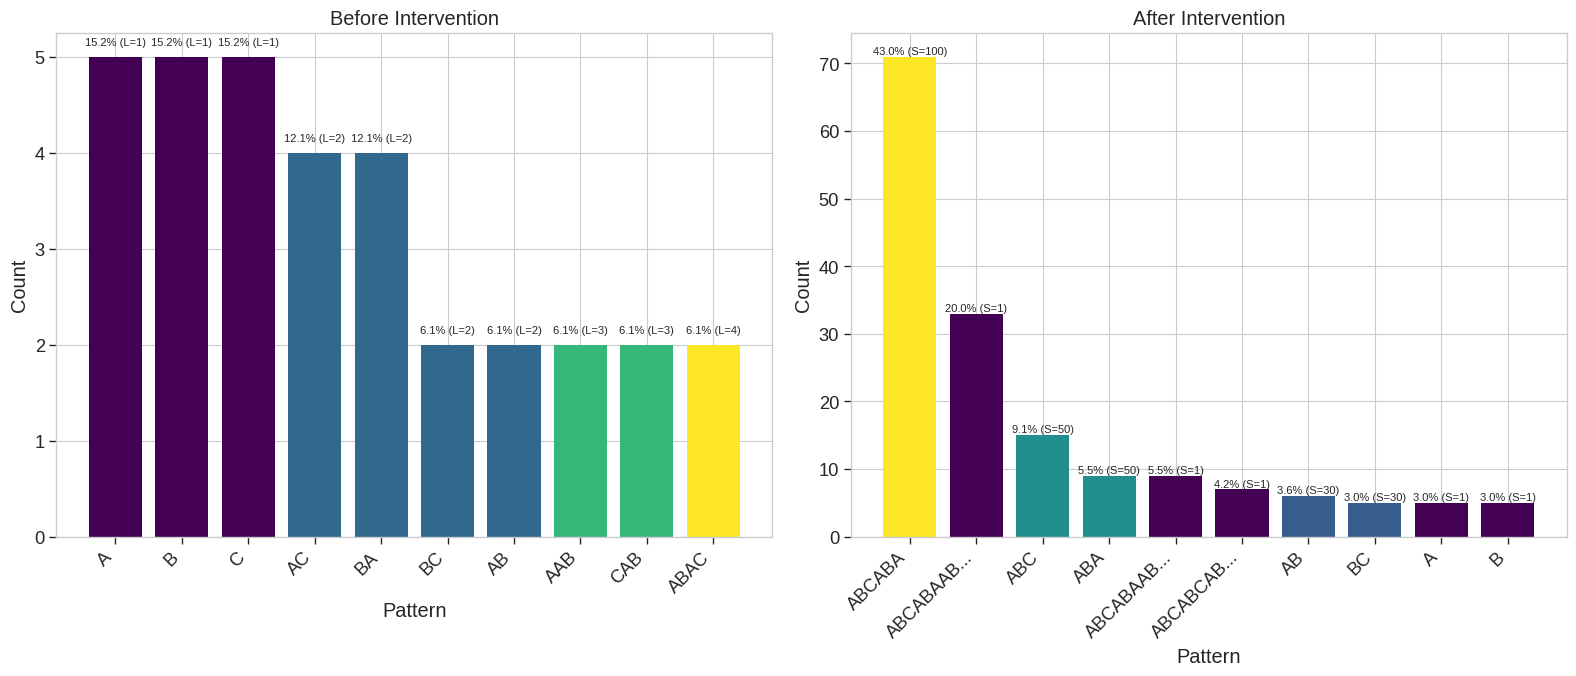
\includegraphics[width=1\textwidth,height=0.55\textwidth]{figure_7.png}
    \caption{Reaction graph for possible Carbon Nanostructure Assembly}
    \label{fig:figure_7}
\end{figure}

Figure~\ref{fig:figure_7} illustrates an abstract reaction graph showing the progressive assembly of carbon-based structures, starting from simple carbon monomers (\( \text{C} \)) and hydrogen atoms (\( \text{H} \)). In the early stages, carbon atoms bond to form dimers (\( \text{C}_2 \)) or small hydrocarbons such as ethylene (\( \text{C}_2\text{H}_4 \)). Through additional interactions and stabilization processes, these smaller molecules transform into increasingly complex structures, such as benzene (\( \text{C}_6\text{H}_6 \)), which serves as a precursor for planar graphene sheets (\( \text{C}_n \)). Ultimately, graphene sheets curl into carbon nanotubes (\( \text{C}_n\text{H}_m \)), high-stability configurations characterized by their exceptional mechanical and electrical properties. 

The main pathway emphasizes the gradual increase in structural complexity and stability. Alongside this progression, less stable intermediates, such as defective graphene or transient molecules, may arise, but typically do not persist due to lower stability. These transient species reflect pathways that are accessible in the reaction space, but are pruned over successive iterations. Here, stability \( S(p) \) plays a central role in determining the persistence and influence of each compound. Simple elements (\( \text{C} \), \( \text{H} \)) and early products (\( \text{C}_2 \), \( \text{C}_2\text{H}_4 \)) possess baseline stability values, representing their shorter lifetimes and higher turnover rates. As more complex compounds are formed, their stability parameters increase, reflecting stronger bonding, lower dissociation rates, and greater resistance to perturbation. Generational updates in a SDSA model dynamically favor the accumulation of these high-stability patterns, leading to the dominance of advanced nanostructures. In contrast, low-stability pathways fade over time, illustrating how stability-driven selection sculpts the molecular landscape and guides the emergence of ordered, complex systems.


\begin{figure}[h]
    \centering
    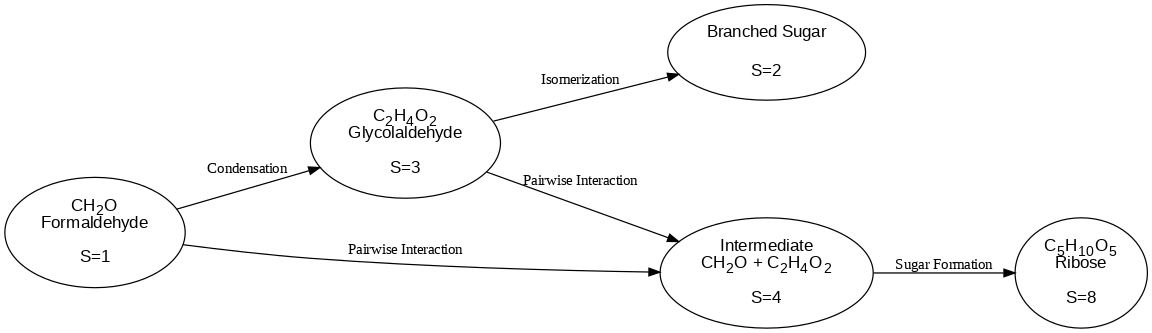
\includegraphics[width=1\textwidth,height=0.4\textwidth]{figure_8.png}
    \caption{Reaction graph for possible pre-RNA Sugar Assembly}
    \label{fig:figure_8}
\end{figure}

Figure~\ref{fig:figure_8} illustrates a simplified reaction network in which small carbonyl-containing molecules, such as formaldehyde (CH$_2$O), undergo pairwise interactions to form sugars of increasing complexity. The pathway begins with the condensation of formaldehyde into glycolaldehyde (C$_2$H$_4$O$_2$), which can interact further to form intermediate compounds, such as a dimer of formaldehyde and glycolaldehyde. These intermediates then serve as precursors to ribose (C$_5$H$_{10}$O$_5$), a key sugar and a crucial building block for RNA. Alongside the main reaction pathway, side reactions lead to the formation of less stable by-products, such as branched sugars, which typically dissipate due to their lower persistence.

These two examples from organic chemistry highlight how stability may play a role in complex reaction graphs. The SDSA perspective supplements conventional kinetic modeling by focusing on net generational outcomes and selective retention, rather than detailing every reversible step. In doing so, SDSA systems reveal how certain ``attractor'' molecules or assemblies can emerge in an otherwise large and branching reaction space, reinforcing the view that stability-driven selection is a powerful force in shaping molecular evolution. However, it is important to acknowledge the limitations of isolating stability as the sole selection factor. In physical systems, molecular persistence is influenced not only by intrinsic stability but also by energy barriers, temperature, catalytic effects, reaction kinetics, and external environmental constraints. Although SDSA systems provide a useful conceptual model, more research is required to quantify the relative contribution of stability compared to other physical and chemical influences in determining the persistence and evolution of molecular structures.



\end{document}

\endinput
%%
%% End of file `elsarticle-template-num.tex'.
